%!TEX root = ../2019_06_04-HATS-LPC-JEC.tex

\subsection{Pileup Reweighting}
%---------------------------------------------------------------------------------------------------------------------------------------
\begin{frame}
    \begin{block}{}
        \begin{center}
            \shadowoffset{2pt}
            \shadowcolor{CUGold}
            \shadowtext{{\fontsize{30}{60}\selectfont \textbf{\textcolor{black}{Pileup Reweighting}}}}
            \vspace{1.5mm}
        \end{center}
    \end{block}
\end{frame}

\begin{frame}[t]\frametitle{Pileup Generation Mechanism}
	\begin{textblock}{0.5}(0.02,0.1)
		\begin{block}{}
			\begin{customlist}{2.5em}{0em}
		    	\item \textbf{Start with chosen input distribution} -- the instantaneous luminosity for a given event is sampled from this distribution to obtain the mean number of interactions in each beam crossing
			    \item the number of interactions for each beam crossing that will be part of the event (in- and out-of-time) is taken from a poisson distribution with the pre-determined mean
			    \begin{customlist}{2.5em}{0em}
			       \item The input distribution is thus smeared by convolving with a poisson distribution in each bin. This is what the {\color{maroon}observed distribution} should look like after the poisson fluctuations of each interaction
			    \end{customlist}
			\end{customlist}			
		\end{block}
	\end{textblock}
	\begin{textblock}{0.46}(0.54,0.1)
		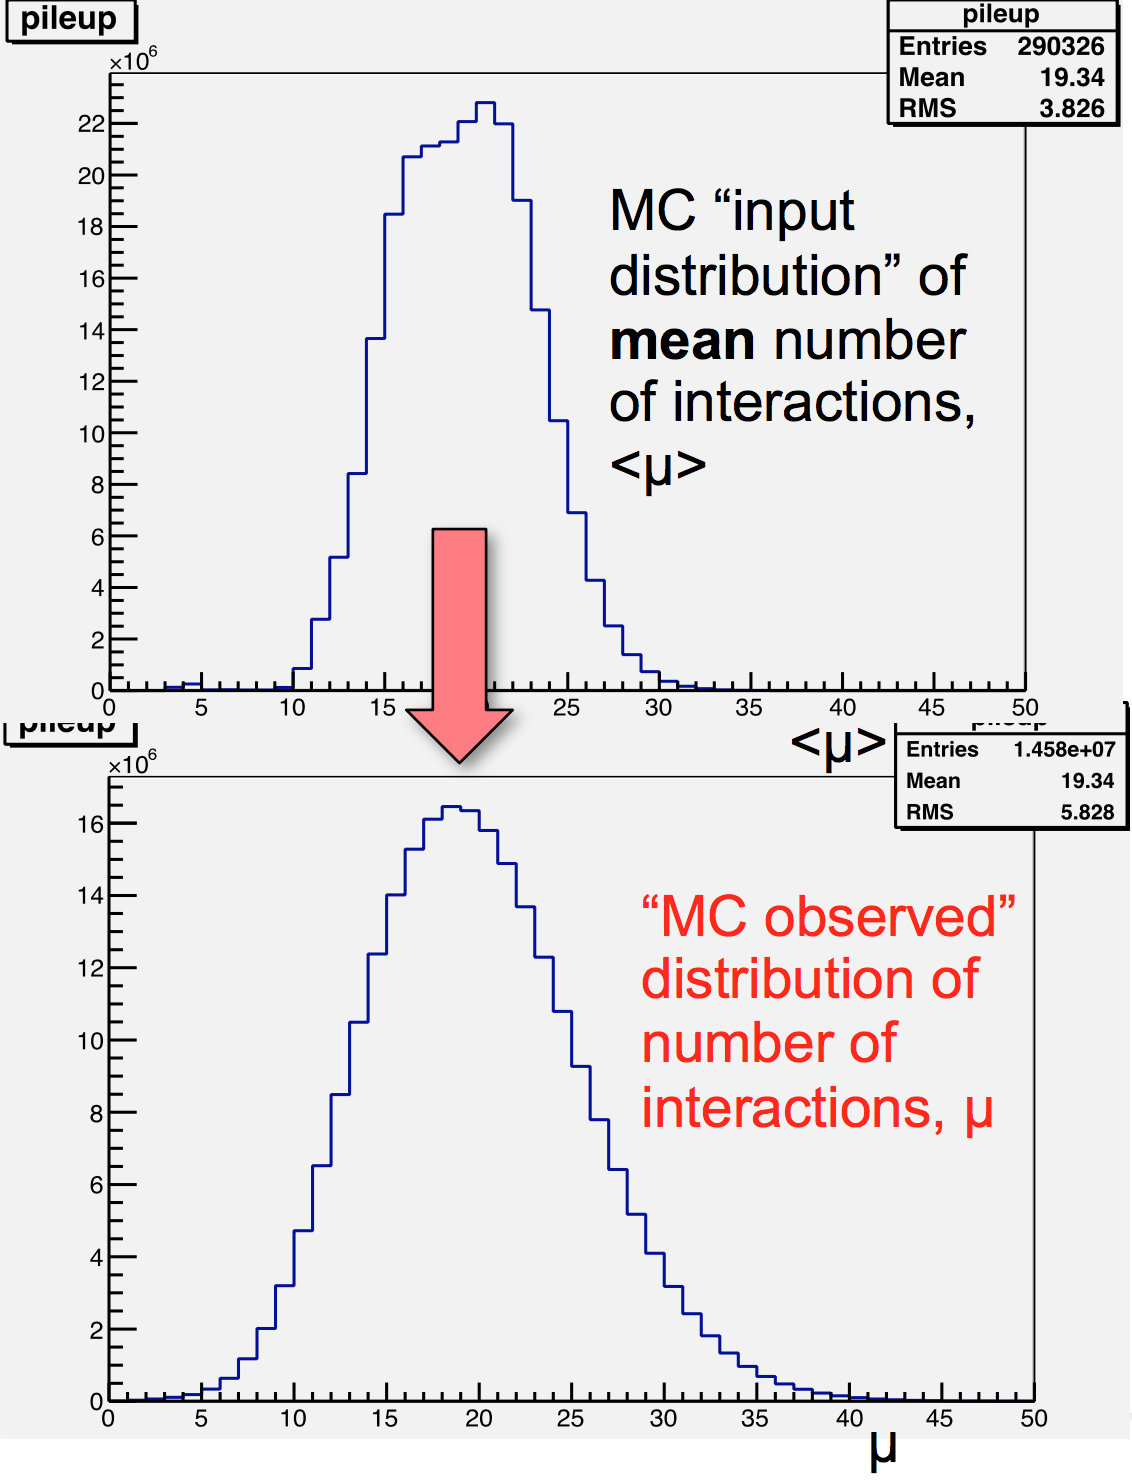
\includegraphics[width=\textwidth]{images/pileup_reweighting/pr_1.png}
	\end{textblock}
\end{frame}

\begin{frame}[t]\frametitle{Pileup Reweighting Procedure}
	\vspace*{-0.35cm}
    \begin{exampleblock}{}
    	\textbf{Goal:} Match generic MC distribution to specific one from data\\
    	\textbf{Example:} Flat10+Tail distribution used for Summer11 MC can be reweighted to match some data distribution\\~~Simple 1-D example (in-time pileup only)
    \end{exampleblock}
    \vspace*{0.5cm}
    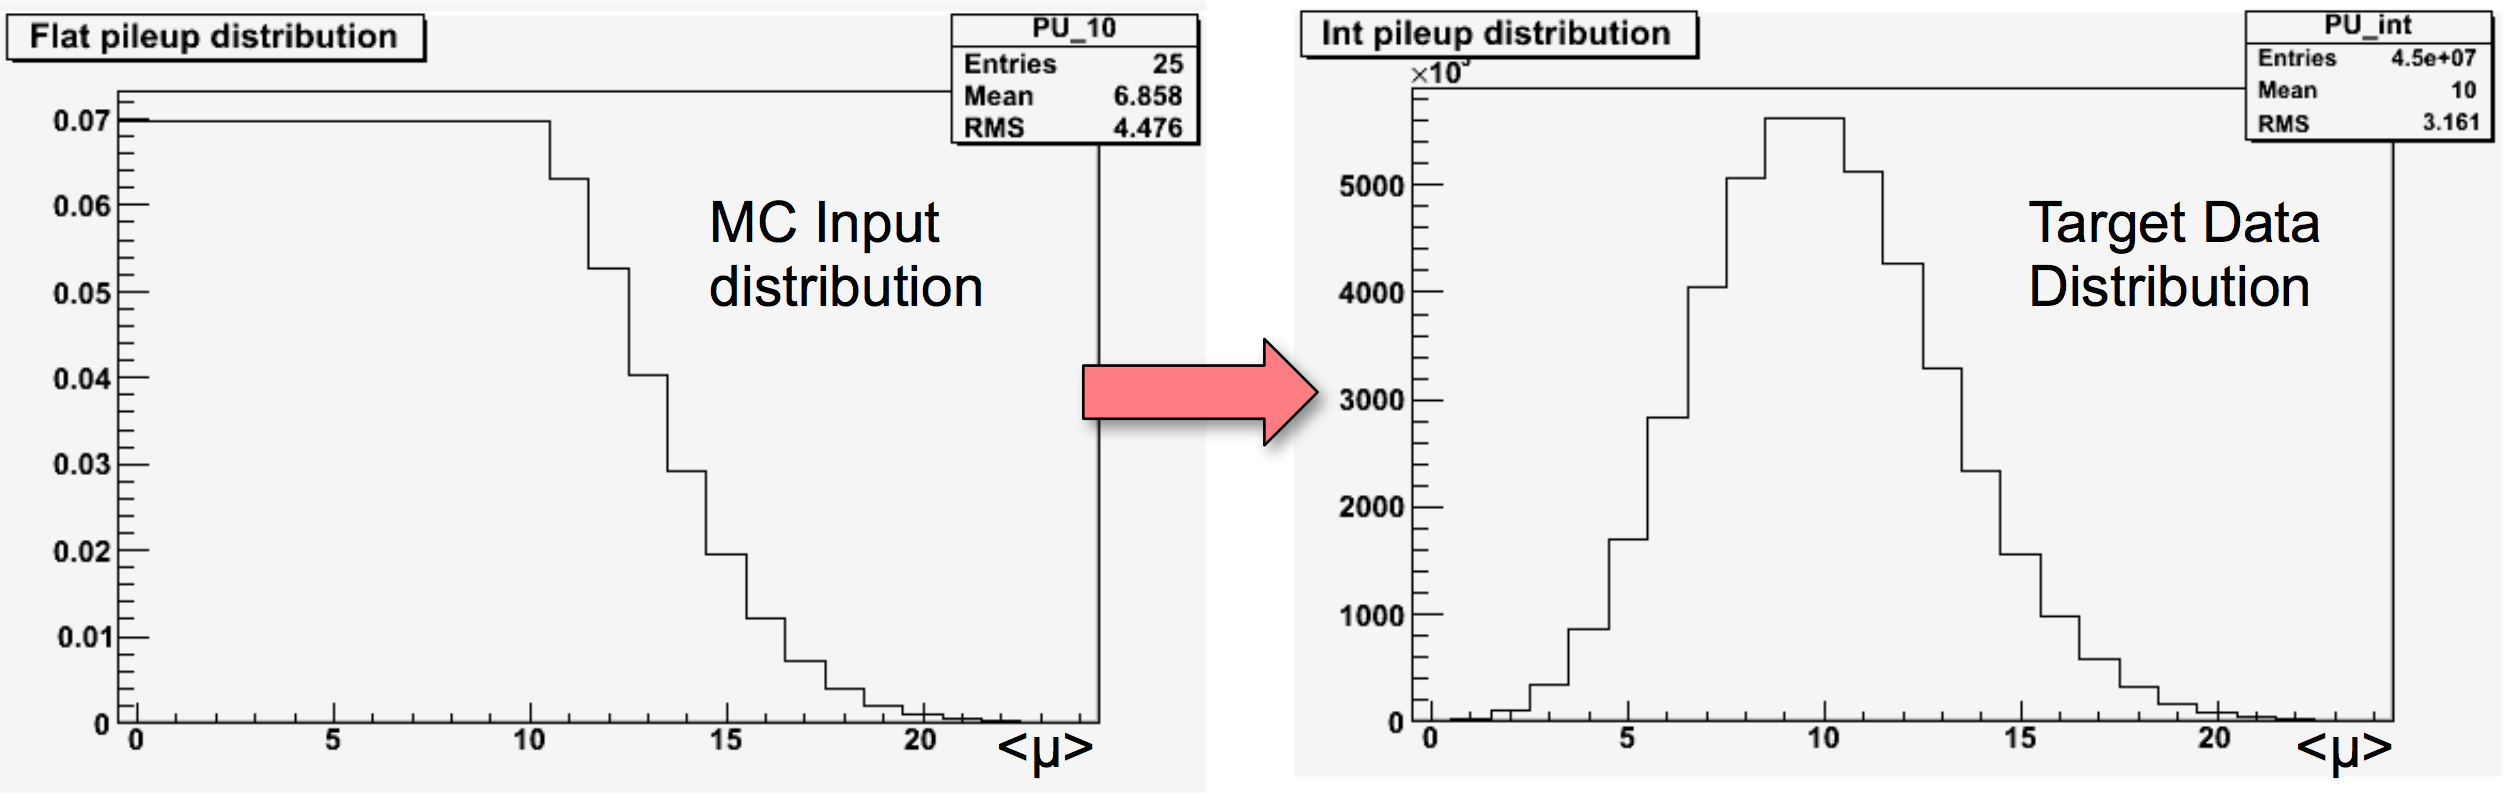
\includegraphics[width=\textwidth]{images/pileup_reweighting/pr_2.png}
\end{frame}

\begin{frame}[t]\frametitle{Pileup Reweighting Procedure}
	\vspace*{-0.35cm}
	\begin{exampleblock}{}
		The ratio of the input and target distributions is used to calculate a weight for each of the input events:
	\end{exampleblock}
	\vspace*{0.25cm}
	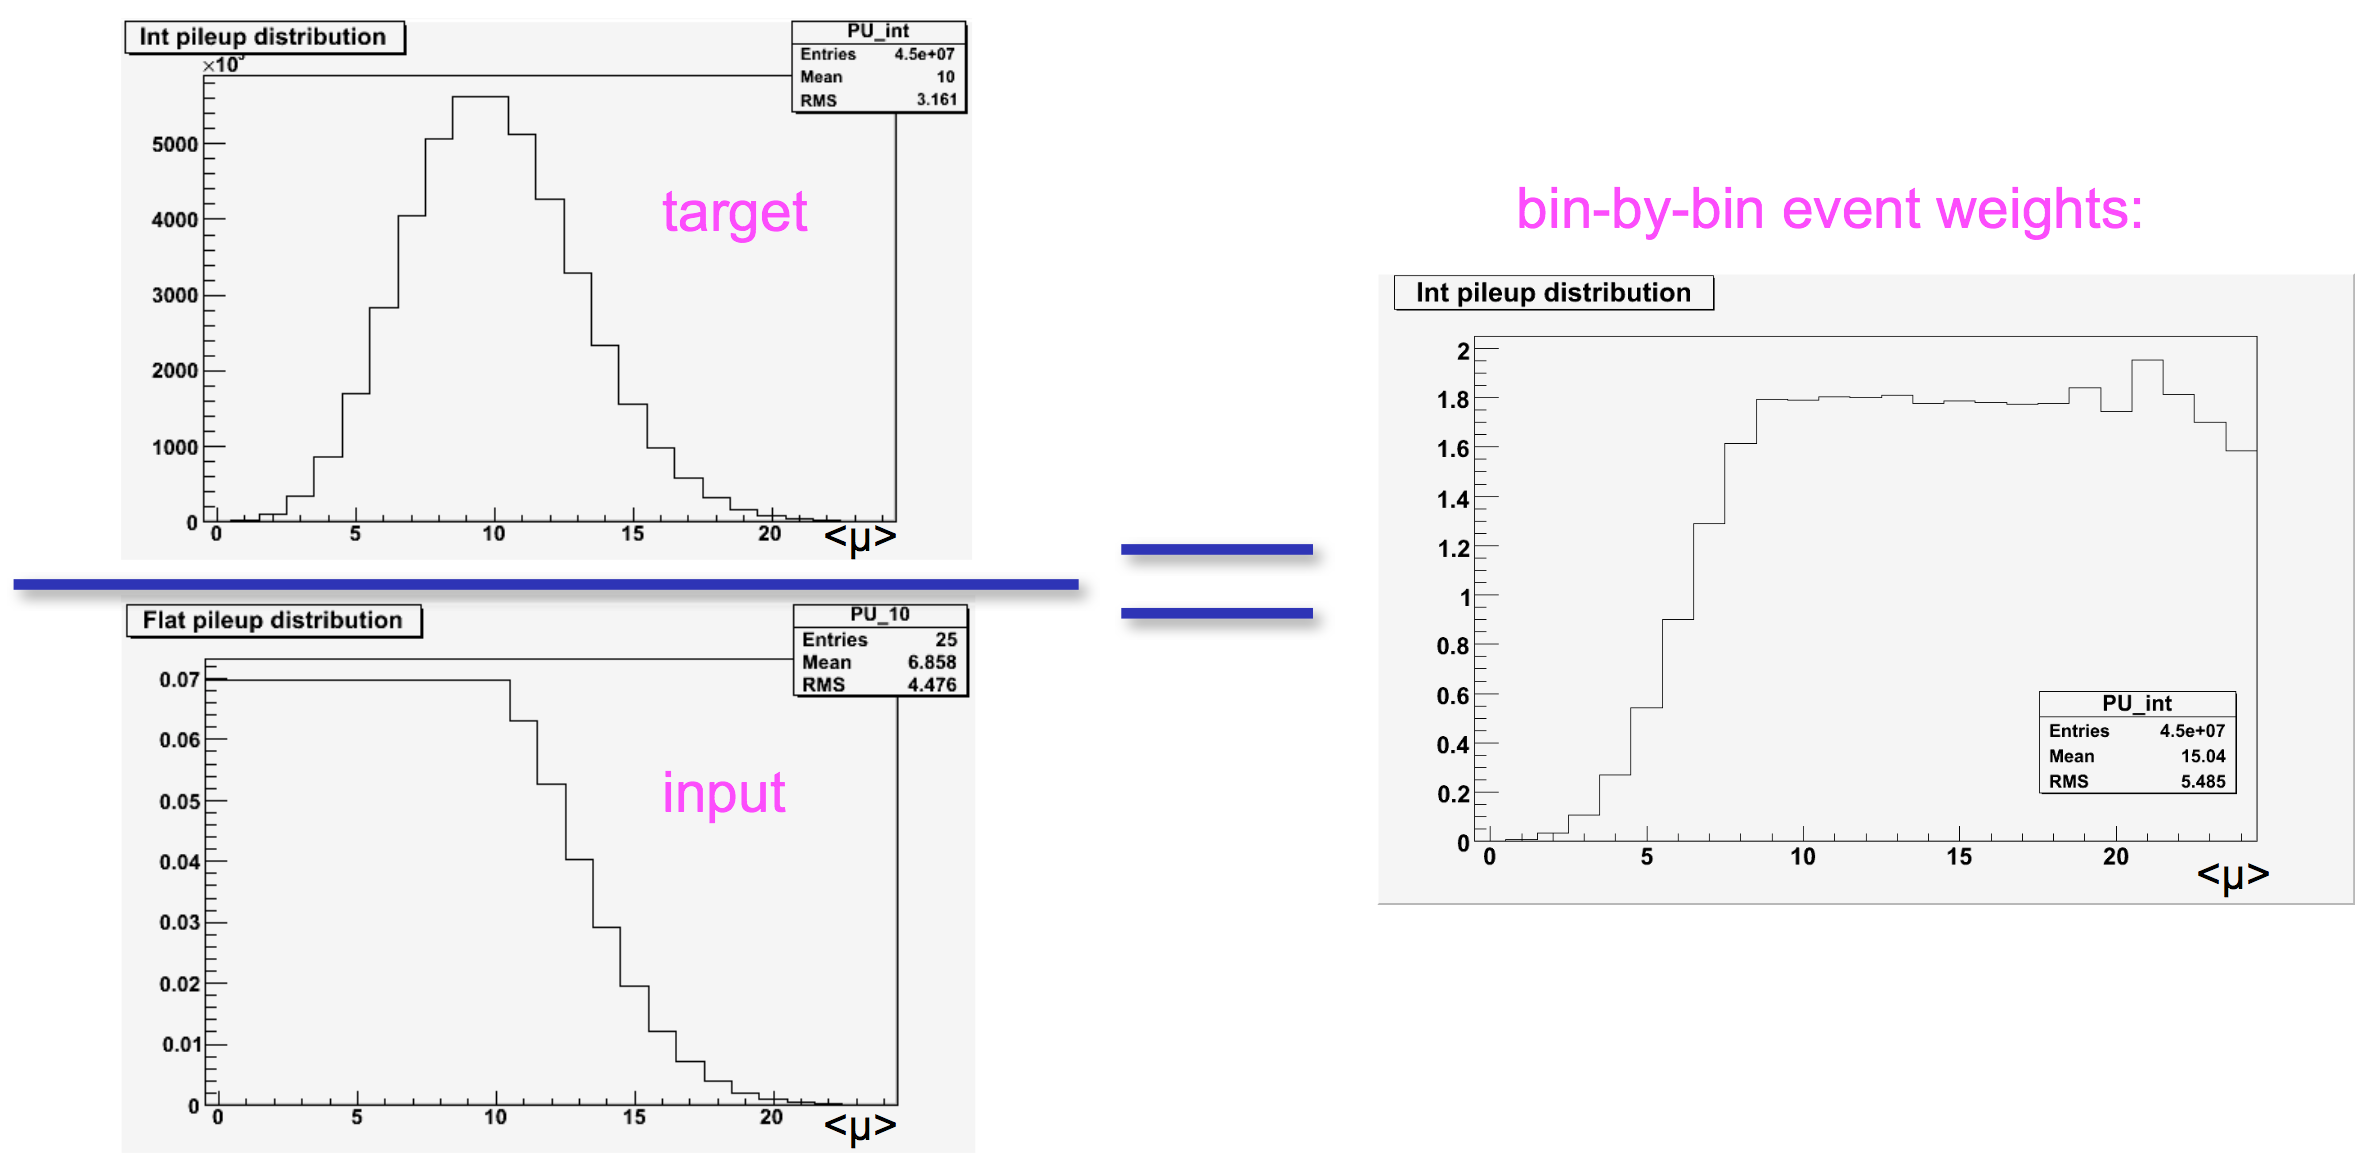
\includegraphics[width=\textwidth]{images/pileup_reweighting/pr_3.png}
\end{frame}

\begin{frame}[t]\frametitle{Pileup Reweighting Procedure}
	\vspace*{-0.35cm}
	\begin{exampleblock}{}
		Then, a MC sample with the same input distribution can be re-plotted with the event weights applied:
	\end{exampleblock}
	\vspace*{0.25cm}
	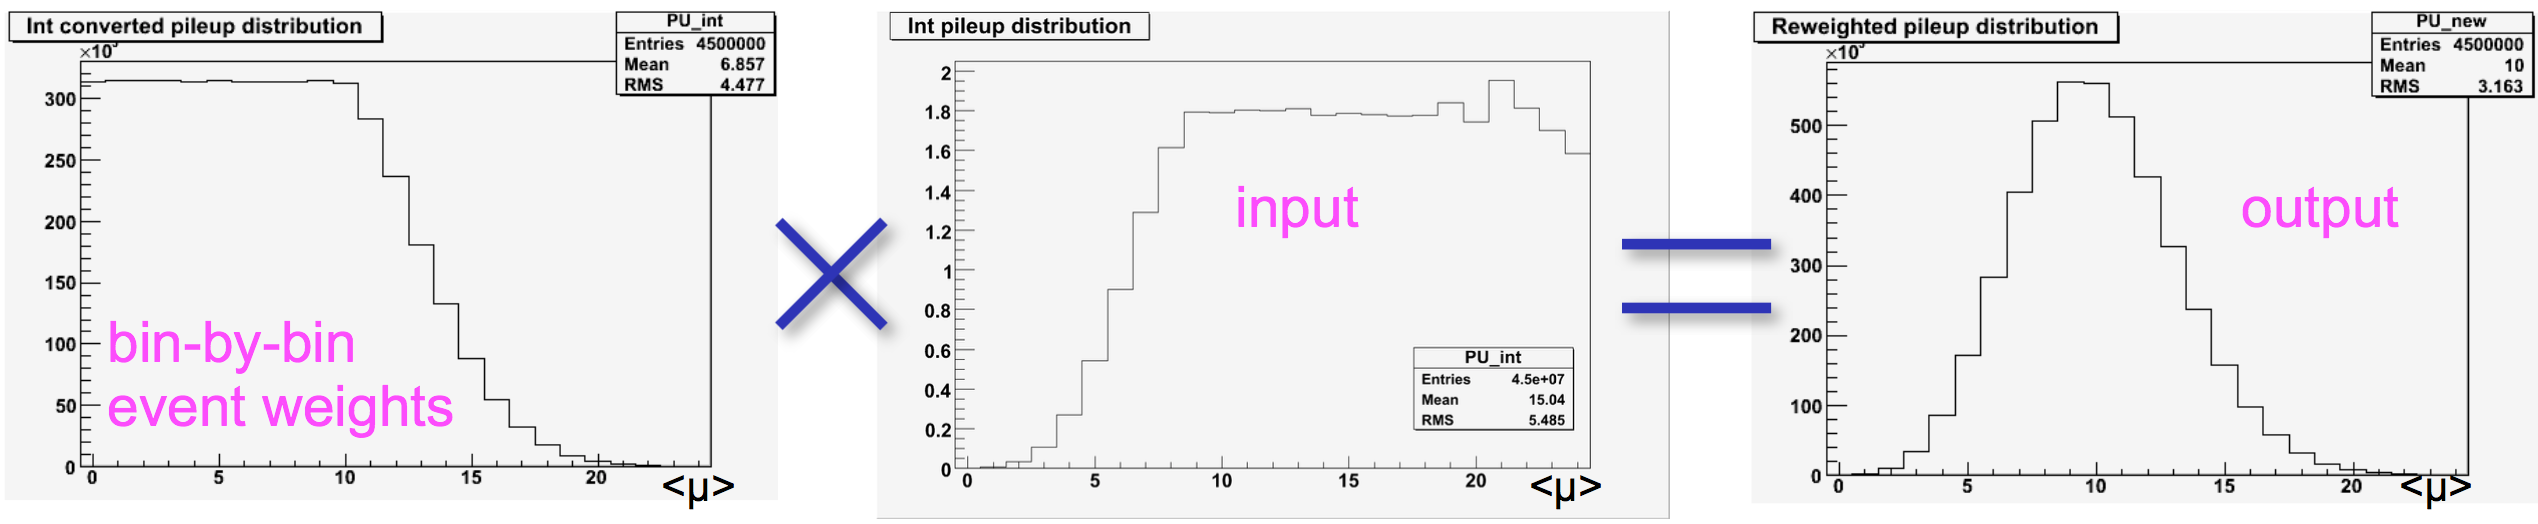
\includegraphics[width=\textwidth]{images/pileup_reweighting/pr_4.png}\\
	\vspace*{0.25cm}
	\hspace*{1.5cm}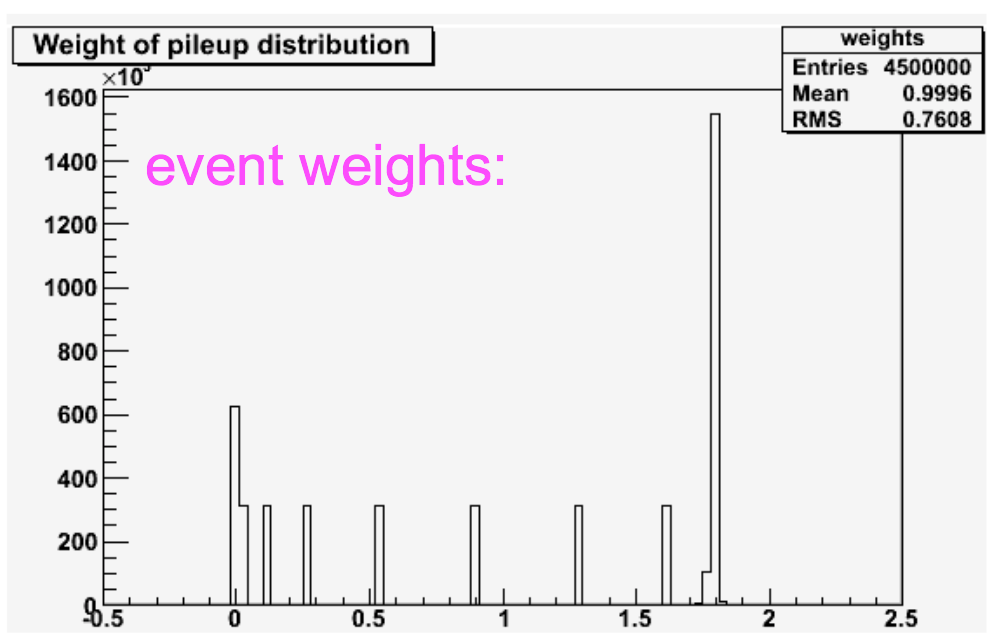
\includegraphics[width=0.32\textwidth]{images/pileup_reweighting/pr_5.png}
	\begin{textblock}{0.5}(0.45,0.6)
		\begin{itemize}
			\item Average event weight is very close to one for this ideal case
			\item May not be true after cuts, since the cuts can bias the MC distribution away from the ideal input
		\end{itemize}
	\end{textblock}
\end{frame}